\documentclass[conference]{IEEEtran}
%\IEEEoverridecommandlockouts
% The preceding line is only needed to identify funding in the first footnote. If that is unneeded, please comment it out.
\usepackage{cite}
\usepackage{amsmath,amssymb,amsfonts}
\usepackage{algorithmic}
\usepackage{graphicx}
\usepackage{textcomp}
\usepackage{xcolor}

%\usepackage{longtable}
%\usepackage{supertabular}
\usepackage{xtab}%,afterpage}
\usepackage{multicol}
\usepackage{pbox}


\def\BibTeX{{\rm B\kern-.05em{\sc i\kern-.025em b}\kern-.08em
    T\kern-.1667em\lower.7ex\hbox{E}\kern-.125emX}}
    
\bibliographystyle{IEEEtran}

\begin{document}

\title{A Review on Intersection Management Systems and recent IoT Integrated Approaches
%\thanks{Identify applicable funding agency here. If none, delete this.}
}

\author{\IEEEauthorblockN{1\textsuperscript{st} Gustavo Velasco-Hernandez}
\IEEEauthorblockA{\textit{School of Electrical and Electronics Engineering} \\
\textit{Universidad del Valle}\\
Cali, Colombia \\
velasco.gustavo@correounivalle.edu.co}
\and
\IEEEauthorblockN{2\textsuperscript{nd} Eduardo Caicedo-Bravo}
\IEEEauthorblockA{\textit{School of Electrical and Electronics Engineering} \\
\textit{Universidad del Valle}\\
Cali, Colombia \\
eduardo.caicedo@correounivalle.edu.co}
}

\maketitle

\begin{abstract}
Intersections or junctions are critical points in transportation systems due to their dynamic behaviour, making them prone to safety or efficiency problems. For this reason, the use of technology in monitoring intersections has increased over the last years. In addition, different proposals based on the Internet of Things (IoT) have been used to handle different traffic issues at intersections, taking advantage of the features it provides regarding hardware, software and communications. This work presents a comprehensive review on Intersection Management Systems (IMS), from a component-based point of view, and a special remark on how IoT-based solutions have been adopted recently in this area is presented as well.
\end{abstract}

\IEEEpeerreviewmaketitle

%\begin{IEEEkeywords}
%component, formatting, style, styling, insert
%\end{IEEEkeywords}

\section{Introduction}
Traditionally, the vision of transport systems has been constrained to the set of elements belonging to infrastructure and the vehicles using it. As population increases and cities grow, the number of vehicles using roads also increases, but the growth rate of the road network is lower. This situation leads to low quality in transportation; congestion and collisions affect mobility in all cities in the world and the development of efficient and long-lasting solutions carry high costs.

The aim of Intelligent Transportation Systems is to address these issues by taking advantage of improvements in information and communication technologies. These ITS include a wide range of applications and services transversal to many knowledge areas. For classifying those services, some taxonomies have been proposed like the ones presented in \cite[Ch.1]{Sussman2005} and \cite{Williams2008}. From described categories and classes, Advanced Traffic Management Systems have to be considered when an intelligent handling of traffic needs to be deployed.

One of the most desirable scenarios to improve efficiency and safety is an intersection. This because intersections are places where vehicles arrive from different directions at different velocities, increasing the chances for incidents and crashes. Choi \cite{Choi2010} states that 40\% of reported traffic accidents in the US were intersection related. Also, in  \cite{CorporacionFondodePrevencionVial2010}, is reported that for Colombia in 2011, most of the accidents in the main cities were at intersections.

On the other side, the Internet of Things has enabled the creation of new sources of data due to the development of low-cost and low-power devices. In addition, the computing capabilities of those devices are increasing constantly, allowing the implementation of complex applications in different areas. One of the areas where IoT-based solutions are integrated is transportation, with great adoption in the intersection management systems field.

In section II, a general description and a review on intersection management systems are presented, from early developments until recent works. Section III describe how IoT-based solutions have been adopted into the field of transportation, specially for optimisation and control at intersections. Finally, in section IV some comments are given and future steps in the area are discussed.

\begin{table*}[tp]
\footnotesize
\caption{Components of an Intersection Management System application.}
\label{imsComps}
\begin{xtabular*}{\textwidth}{|c|c|c|c|c|}
\hline
\textbf{Application} & \textbf{Data Source} & \textbf{Target} & \textbf{Communication} & \textbf{Implementation}\\
\hline
\parbox{3.8cm}{
Monitoring:
\begin{itemize}
	\item Recognition
	\item 		Detection
	\item 			Tracking
\end{itemize}
Control:
	\begin{itemize}
		\item Traffic control
		\item 			Warning advertisement
		\item 			Traffic rules supervision
	\end{itemize}
	Analysis:
	\begin{itemize}
		\item Traffic flow
		\item 			Path analysis
		\item 			Context and behavior
	\end{itemize}
	}
 & 
 \parbox{3cm}{
 Infrastructure:
 \begin{itemize}
		\item Presence sensors
		\item			Range sensors
		\item			Image sensors 
		\item			RFID and wireless
	\end{itemize}
 	
		Vehicle:
			
		\begin{itemize}
		\item Position
		\item 			State 
		\item 			Travel information	 

	\end{itemize}
	}
&
 \parbox{2.5cm}{	 
	\begin{itemize}
		\item Pedestrians
		\item 			Bicycles
		\item Motorcycles
		\item 			Small Vehicles
		\item 			Large Vehicles
	\end{itemize}
	}
&
 \parbox{3.8cm}{	 
	\begin{itemize}
		\item V2V - Vehicle-to-vehicle
		\item 			V2I - Vehicle-2-vehicle
		\item 			V2X - Vehicle to anything 
	\end{itemize}
	}
&
\parbox{2.9cm}{	 
	\begin{itemize}
		\item Real
		\item 			Simulation
		\item 			Augmented Reality
		\item 			Dataset
		\item 			Scale-model
	\end{itemize}
	} \\
\hline

%\end{xtabular*}
%\end{table*}
\end{xtabular*}
\end{table*}

\section{Intersection Management Systems}



Different types of applications and systems are conceived to address these issues. Some tasks performed by those systems are intersection monitoring, vehicles detection, incident warning, collision avoidance, among others. A typical Intersection Management System is composed by three main components: Data source, that could be infrastructure sensors, like inductive loops, range sensors or cameras, and vehicle sensors and traveling data; decision system, which is the core of the whole system, is in charge of analyse and process information provided by infrastructure, vehicles and authorities in order to identify objects, recognise patterns, predict future incidents, control traffic and generate safe decisions and warnings alerts; and finally, is the presentation and displaying of the output of decision system, through infrastructure using dynamic signals, traffic light controlling, or using direct communication with drivers or vehicles through on-board visualisation/notification system. A block diagram of a generic IMS is presented in figure \ref{arch}

\begin{figure}[ht!]
\centering
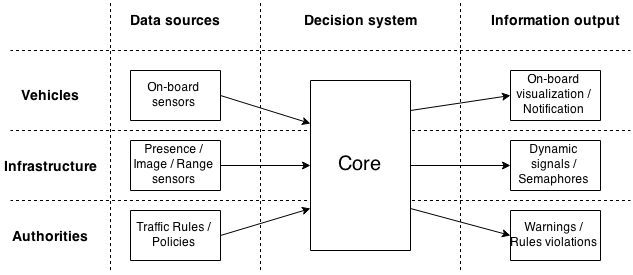
\includegraphics[scale=0.38]{../fig/2/genericIMS.png}
\caption{Generic block diagram of an Intersection Management System.}
\label{arch}
\end{figure}

\subsection{Components in IMS application}

Intersection monitoring is a required task to be done within intelligent transportation systems for high-level applications like traffic analysis, counting and classification of vehicles or pedestrians, event prediction, incident detection and security and surveillance systems. Those applications have to take into account some of the elements depicted in figure \ref{arch} and developments in IMS have a wide range of approaches and objectives. In order to study IMS applications, five components have been defined which are present on those applications, and on most cases, more than one component could be involved in the same development. Table \ref{imsComps} describe aforementioned components and elements within them along with a brief description.



%INTERSECTION MANAGEMENT SYSTEM	Application	Monitoring	Recognition
%			Detection
%			Tracking
%		Control	Traffic control
%			Warning advertisement
%			Traffic rules supervision
%		Analysis	Traffic flow
%			Path analysis
%			Context and behavior
%	Data source	Infrastructure	Presence sensors
%			Range sensors
%			Image sensors 
%			RFID and wireless
%		Vehicle	Position
%			State 
%			Travel information
%	Target		Pedestrians
%			Bicycles / Motorcycles
%			Small Vehicles
%			Large Vehicles 
%	Communication		V2V -Vehicle -to-vehicle
%			V2I - Vehicle-2-vehicle
%			V2X
%	Implementation		Real
%			Simulation
%			Augmented Reality
%			Dataset
%			Scala-model


\subsubsection{Application}

Application component could be seen as the final objective of the system. Generally, this includes high-level tasks like monitoring, analysis or control. Monitoring or surveillance systems execute actions like recognition, detection and/or tracking of objects in the scene. 
Other systems analyse the behaviour and interactions between detected objects to recognise path patterns, determine the context of the environment and predict some events of interest. At a higher level there are systems which make decisions based on detection of certain traffic conditions to handle traffic lights, control intersection access, generate warnings to drivers or issue traffic tickets when a rule violation exists.

\subsubsection{Data Source}

The origin of data is considered an independent component because of the variety of possible sources and posterior processing stages. From infrastructure side, data can be captured using a wide range of sensors like inductive loops, lasers, lidars and cameras. Also, monitoring connections to wireless networks. On the other side, data from vehicles is also useful for the system to enhance its representation of the scene and take decisions. This could be low-level data like vehicle state variables, for example, speed, orientation, acceleration, etc., or high-level data like travel information.


\subsubsection{Target}

In an intersection many objects of different kinds interact between them. Pedestrian and vehicles are found at intersections, and latter includes bicycles, motorcycles, cars, vans, buses, trucks and some other types of vehicles. For this reason some applications are designed for a specific element or group of elements. Pedestrian tracking, motorcycles recognition or car counting are examples of targeted applications.

\subsubsection{Communication}

One of the keypoints of ITS is how information technologies and communication advances are included in transportation. The main goal of this is to allow information sharing between vehicles and infrastructure entities. For this reason, 3 communication approaches appear: Vehicle-to-vehicle or Inter-vehicle communication (V2V), vehicle-to-infrastructure communication (V2I) and vehicle to both vehicle and infrastructure (V2X). Several protocols and standars have been proposed for these communication approaches, for example DSRC, WAVE and IEEE 802.11p, but research and development on this component is still active.

\subsubsection{Implementation}

Not all IMS applications are implementable on a real scenario, maybe because is not the scope of the application or because it is in a early stage and it could be validated in other ways. This types of developments are sometimes implemented and evaluated using simulators, making functional prototypes or deploying scale-models. Some other projects use datasets to evaluate new algorithms and data processing techniques, and then compare obtained results with previous works. Augmented reality is also used as a tool for evaluating and validate developments, taking advantage of the interaction of a real system with a simulated/artificial scenario.

\subsection{Developments in Intersection Management Systems}

In the table \ref{reviewtable} is presented a compilation of several developments within IMS field from the last 10 years. For each work a description is given in which target and implementation components are highlighted. Additionally, Data source, communication and application components are detailed in their own column. 

%\clearpage 
%\onecolumn

% IMS review table
%\begin{center}

%\begin{supertabular} {|c|p{0.3\linewidth}|p{0.15\linewidth}|p{0.1\linewidth}|c|}
%\begin{longtable} {|c|p{0.3\linewidth}|p{0.15\linewidth}|p{0.1\linewidth}|c|}
%\begin{xtabular*}{|c|p{0.3\linewidth}|p{0.15\linewidth}|p{0.1\linewidth}|c|}
%\begin{table}
%\afterpage{
%\onecolumn
%\begin{table}
%\onecolumn
%\begin{xtabular*}{\textwidth}{|p{0.1\textwidth}|p{0.4\textwidth}|p{0.15\textwidth}|p{0.1\textwidth}|p{0.121875\linewidth}|}
%\begin{xtabular*}{\linewidth}{@{\extracolsep{\fill}}|*{5}{p{1.2cm}|}}
%\hline
%\multicolumn{5}{|c|}{ \textbf{Developments on Intersection Management Systems} } \\
%
%\hline
%\pbox{0.1\linewidth}{\textbf{Reference}} & 
%\pbox{0.4\linewidth}{\textbf{Comment}} & 
%\pbox{0.15\linewidth}{\textbf{Application}} & 
%\pbox{0.1\linewidth}{\textbf{Data Source}} & 
%\pbox{0.1\linewidth}{\textbf{Communication}} \\

%\hline
%\endfirsthead
%\hline
%\textbf{Reference} & \textbf{Comment} & \textbf{Application} & \textbf{Data Source} & \textbf{Communication} \\
%\hline
%\endhead

%% IMS review table
\begin{center}
\footnotesize
\begin{longtable}{|c|p{0.3\linewidth}|p{0.15\linewidth}|p{0.1\linewidth}|c|}
%\begin{tabular}
\hline
\multicolumn{5}{|c|}{ \textbf{Developments on Intersection Management Systems} } \\

\hline
\textbf{Reference} & 
\pbox{0.3\linewidth}{\textbf{Comment}} & 
\pbox{0.15\linewidth}{\textbf{Application}} & 
\pbox{0.1\linewidth}{\textbf{Data Source}} & 
\textbf{Communication} \\

\hline
\endfirsthead
\hline
\textbf{Reference} & \textbf{Comment} & \textbf{Application} & \textbf{Data Source} & \textbf{Communication} \\
\hline
\endhead

\cite{Kamijo1999, Kamijo2000} & 
{They show an intersection monitoring system based on a fixed camera. This system is divided in three stages: Background modeling, object tracking and accident detection. They propose an innovative feature for accident detection using HMM.} & 
{Accident  detection} & 
Camera & 
N/A \\
\hline

\cite{Veeraraghavan2002} &
{Passive video-based system for monitoring an intersection. They implemented Stauffer's Method for background modeling, PCA for oriented bounding box computation, and Graph-based tracking and motion estimation. Also a simple methods for classification and calibration are described.} &
{Accident  detection} & 
Camera & 
N/A \\
\hline

%\cite{Gehrig2003} & & & & \\ \hline

\cite{Veeraraghavan2003} &
They present 4 stages for IMS: background modeling, motion tracking, feature extraction, calibration. They propose a 2-level tracking: Blob tracking as low-level and position using Kalman filter as high-level. &
Accident detection / prediction &
Camera & 
N/A \\
\hline

\cite{Messelodi2004} &
A Full implementation of an IMS in a town in northern Italy. The system claims to be independent of intersection geometry and it is based on a monocular camera. Processing stages of the system and classification approaches are described. &
Intersection Monitoring &
Camera &
N/A \\
\hline

\cite{Dogan2004} &
Development of a simulator for an Intersection Collision Warning System. Physical and MAC layers were modeled &
Intersection collision warning simulator &
N/A &
V2V \\
\hline

\cite{Chan2004} &
 Traffic monitoring for two context: Left-Turn-Across-Path-Opposite-Direction and Dilemma zone and red light violation &
Intersection Monitoring &
Radar &
N/A \\
\hline

\cite{Atev2005} &
A collision prediction system based on computational geometry is presented. The two main stages are low-level vision system for foreground optimization, with shaking compensation and noise removal, and a collision prediction system based on bounding boxes instead of bounding rectangles. &
Collision prediction &
Camera &
N/A \\
\hline

\cite{Chan2005} &
Analysis of Left-Turn-Across-Path-Opossite-Direction conflict situation. &
Intersection Monitoring &
Radar; Steering, speed sensors and GPS on-board &
V2X \\
\hline

\cite{Avila2005} &
Based on \cite{Dogan2004}, this works includes and improvement, including network layer and driver behaviour model. &
Intersection Simulator Architecture &
N/A &
V2X \\
\hline

\cite{Veeraraghavan2005} &
Tracking system based on Kalman filter for tracking and event detection at intersections, capable of detect 4 events: Acceleration, uniform velocity, stop and turns. &
Tracking and event detection &
Camera &
N/A \\
\hline

\cite{Zhao2006} &
Object tracking and classification at intersection using a single laser scanner. The system identifies 3 classes: Pedestrians, 2-wheeled vehicle and cars. It is based on points clustering, KL transform and markov chains &
Object tracking and classification &
Laser &
N/A \\
\hline

\cite{Eguchi2007} &
A system for discriminate an approaching vehicle to an intersection is described. It use a monocular camera and define a number of features for classification. Motion vectors are used too and determine the level of approaching. &
Vehicle detection &
Camera &
N/A \\
\hline

\cite{Kuramoto2007} &
A communication scheme based on nearest to intersection is described. Two zones are defined: nearest zone and quasi-nearest zone. Based on which zone vehicles are, communicaton is performed. Validation of proposal is done using a custom microscopic simulator. &
Intersection Communication Scheme &
N/A &
V2I \\
\hline

\cite{Dresner2008} &
A multiagent-based intersection control protocol called autonomous intersection management (AIM) is proposed. Based on a custom simulation, vehicles are modeled and they comunicate with an intersection manager which allows or deny access to intersection. It is possible to set different traffic policies, even for emulate current control approaches lke stop lights and traffic lights. &
Intersection Management &
On-board state sensors &
V2I \\
\hline

\cite{Jarupan2008} &
Based on \cite{Dogan2004} and \cite{Avila2005}, this simulator architecture emphasize on wireless communications. Now the system allows to compare different communication protocols and traffic configurations. &
Intersection Simulator Architecture &
N/A &
V2V \\
\hline

\cite{Zhao2008} &
Based on \cite{Zhao2006}, the system now includes more laser sensor for get a better representation of the scene, solving some occlusion issues. Clustering is used for grouping readings from different sensors belonging to the same object and a tracking approach based on angle of beam, range and time is presented. &
Intersection monitoring &
Lasers &
N/A \\
\hline

\cite{Rawashdeh2008} &
Proposal of a communication architecture for vehicles approaching to an intersection. Two zones are defined: Control Channel Zone (CCHZ) and Service Channel Zone (SCHZ). Also, 3 different methods are described for the system to be implmented &
Collision avoidance &
N/A &
V2I \\
\hline

\cite{Mundewadikar2008} &
Proposal of a physical-layer protocol for V2I communication at intersections. The system is evaluated in simulation using MATLAB &
Collision detection and warning &
N/A &
V2I \\
\hline

\cite{Zhao2009} &
Based on \cite{Zhao2008}, now the system includes a camera for video capture. In this video, data obtained from the lasers-based system are projected, drawing bounding boxes for vehicles and lines for trajectories. &
Intersection monitoring &
Camera, Lasers &
N/A \\
\hline

\cite{Abbas2009} &
Monitoring dilemma zone and efectiveness of control policies using cameras and loop detectors on an intersection &
Intersection monitoring &
Cameras, loop detectors &
N/A \\
\hline

\cite{Babaei2010} &
Author presents a system for foreground extraction, vehicle detection and tracking. A novel algorithm is proposed based on image division in traffic zones to perform background removal and vehicle detection. This proposal is compared with traditional MoG approach. &
Intersection monitoring &
Camera &
N/A \\
\hline

\cite{Meissner2010} &
A semi-automatic calibration method for a network of lidar sensors is presented using a custom simulation environment. Also, a calibration object were designed based on simulation results. &
Intersection Monitoring &
Lidars &
N/A \\
\hline

\cite{Quinlan2010} &
An augmented reality implementation of the system proposed in cite{Dresner2008} is presented. In this work, an autonomous vehicle is deployed in a mixed-reality platform and request to an virtual intersection manager for authorisation to cross and is the manager which decides if it is safe to cross or not, depending on the defined traffic policies and the state of virtual vehicles. &
Intersection management &
On-board state sensors &
V2I \\
\hline

\cite{Ball2010} &
The use of intelligent objects in vehicles is proposed. With sharing vehicle state information and jouney plans, the system aims to better control traffic in intersection using a novel back-off protocol instead of time traffic control system. &
Traffic control &
On-board state sensors, Journey plans &
V2V \\
\hline

\cite{Babaei2011} &
A system for traffic flow measurement based on anormalities detection is presented. Multiple cameras are used SIFT and unsupervised SVM-based clustering are performed for trajectories analysis. &
Intersection monitoring &
Cameras &
N/A \\
\hline

\cite{Basma2011} &
In presented system, wireless magnetic nodes are used to detect presence and to send data to a base station, which determines possible collisions and warns driver through a visualisation system in infrastructure. &
Collision Avoidance	 &
Presence sensors &
N/A \\
\hline

\cite{Azimi2012} &
An intersection control protocol based on V2V communication is proposed. This protocol is in charge of handling other vehicles messages and determines if is it safe or not to cross. They present two policies for managing intersection access: Concurrent Crossing- Intersection Protocol (CC-IP) and Maximum Progression-Intersection Protocol (MP-IP). &
Intersection management &
N/A &
V2V \\
\hline

\cite{CondeBento2012} &
A microscopic simulator was developed, with a spatial-temporal-based approach for managing the intersection. It is possible to implement different traffic policies for comparison purposes and the system works on crossroads and roundabouts. &
Intersection management &
On-board state sensors &
V2X \\
\hline

\cite{Zhao2012} &
A novel approach for detecting moving objects and track them is presented. The focus of this work relies on process merged data from laser sensors (\cite{Zhao2009}) to get better results at tracking. &
Object detection and tracking &
Lasers &
N/A \\
\hline

\cite{Jin2012} &
A Multiagent-based system is proposed. They define a Vehicle Agent and and Intersection Agent and propose a protocol for controlling intersection access based on timeslots, Also, the present a vehicle motion planning algorithm. Validation and testing was done using SUMO platform &
Intersection Management &
On-board state sensors &
V2I \\
\hline

\cite{Meissner2012} &
A set of laser scanners is used for detect and track pedestrians. GMM and DBSCAN are proposed for detection stage. For tracking purpose, a random finite set particle filter is used. &
Pedestrians detection and tracking &
Lasers &
N/A \\
\hline

\cite{Goldhammer2012} &
In this work is presented the setting and configuration of a multisensor network, based on 14 lasers, 10 cameras, GPS and V2I unit. Calibration and spatial-temporal alignment is performed. &
System Architecture &
Cameras, Lasers &
V2I \\
\hline

\cite{Friesen2013} &
A set of wireless probes are deployed to estimate traffic flow based on bluetooth connections. Then, using Zigbee, data is send to a master node which handle data for forwarding to a server / database for further processing. &
Traffic monitoring &
Wireless sensor network &
N/A \\
\hline

\cite{Guerrero-Ibanez2013} &
Two modes of Intersection Access Control: V2I mode and V2V mode. Implementation was done using minirobots in a scale model of an intersection. &
Intersection access control &
Loop detectors and RFID nodes &
V2X \\
\hline

%\cite{Meissner2013,Meissner2013a} &
% &
% &
% &
% \\
%\hline

\cite{Meissner2013b} &
A new method for object detection based on lidars data is proposed. After perform background removal, they use DBGridSCAN for 3D clustering and 2D pathway tracking. Then a combination of 2D-3D is done. The proposal is validated using OSPA metric. &
Object Detection &
Lasers &
N/A \\
\hline

\cite{Au2015} &
On top of AIM (\cite{Dresner2008}) Semi-AIM protocol is proposed. Assuming that human-driven vehicles to autonomous vehicles transition will be long, this system is intended for semi-autonomous vehicles. Also the author describe the human relation to a semi-autonomous vehicle and analyse how the features of autonomy employed by the car affects the traffic delay. &
Intersection Management &
On-board state sensors &
V2I \\
\hline

%\cite{} &
% &
% &
% &
% \\
%\hline

%\cite{} &
% &
% &
% &
% \\
%\hline

%\cite{} &
% &
% &
% &
% \\
%\hline

%\cite{} &
% &
% &
% &
% \\
%\hline

%\cite{} &
% &
% &
% &
% \\
%\hline

%\cite{} &
% &
% &
% &
% \\
%\hline


\hline
%\end{tabular}
\caption{Developments related to Intersection Management Systems.}
\label{reviewtable}
\end{longtable}
\end{center}

%\begin{table*}[tp]
%\caption{Developments on Intersection Management Systems}
%\label{reviewtable}
%\begin{xtabular*}{\textwidth}{|p{0.08\textwidth}|p{0.41\textwidth}|p{0.15\textwidth}|p{0.12\textwidth}|p{0.121875\linewidth}|}
%
%\hline
%\textbf{Reference} & \textbf{Comment} & \textbf{Application} & \textbf{Data Source} & \textbf{Communication} \\
%\hline
%
%
%\cite{Kamijo1999, Kamijo2000} & 
%{They show an intersection monitoring system based on a fixed camera. This system is divided in three stages: Background modeling, object tracking and accident detection. They propose an innovative feature for accident detection using HMM.} & 
%{Accident  detection} & 
%Camera & 
%N/A \\
%\hline
%
%\cite{Veeraraghavan2002} &
%{Passive video-based system for monitoring an intersection. They implemented Stauffer's Method for background modeling, PCA for oriented bounding box computation, and Graph-based tracking and motion estimation. Also a simple methods for classification and calibration are described.} &
%{Accident  detection} & 
%Camera & 
%N/A \\
%\hline
%
%%\cite{Gehrig2003} & & & & \\ \hline
%
%\cite{Veeraraghavan2003} &
%They present 4 stages for IMS: background modeling, motion tracking, feature extraction, calibration. They propose a 2-level tracking: Blob tracking as low-level and position using Kalman filter as high-level. &
%Accident detection / prediction &
%Camera & 
%N/A \\
%\hline
%
%\cite{Messelodi2004} &
%A Full implementation of an IMS in a town in northern Italy. The system claims to be independent of intersection geometry and it is based on a monocular camera. Processing stages of the system and classification approaches are described. &
%Intersection Monitoring &
%Camera &
%N/A \\
%\hline
%
%\cite{Dogan2004} &
%Development of a simulator for an Intersection Collision Warning System. Physical and MAC layers were modeled &
%Intersection collision warning simulator &
%N/A &
%V2V \\
%\hline
%
%\cite{Chan2004} &
% Traffic monitoring for two context: Left-Turn-Across-Path-Opposite-Direction and Dilemma zone and red light violation &
%Intersection Monitoring &
%Radar &
%N/A \\
%\hline
%
%\cite{Atev2005} &
%A collision prediction system based on computational geometry is presented. The two main stages are low-level vision system for foreground optimization, with shaking compensation and noise removal, and a collision prediction system based on bounding boxes instead of bounding rectangles. &
%Collision prediction &
%Camera &
%N/A \\
%\hline
%
%\cite{Chan2005} &
%Analysis of Left-Turn-Across-Path-Opossite-Direction conflict situation. &
%Intersection Monitoring &
%Radar; Steering, speed sensors and GPS on-board &
%V2X \\
%\hline
%
%\cite{Avila2005} &
%Based on \cite{Dogan2004}, this works includes and improvement, including network layer and driver behaviour model. &
%Intersection Simulator Architecture &
%N/A &
%V2X \\
%\hline
%
%\cite{Veeraraghavan2005} &
%Tracking system based on Kalman filter for tracking and event detection at intersections, capable of detect 4 events: Acceleration, uniform velocity, stop and turns. &
%Tracking and event detection &
%Camera &
%N/A \\
%\hline
%
%\cite{Zhao2006} &
%Object tracking and classification at intersection using a single laser scanner. The system identifies 3 classes: Pedestrians, 2-wheeled vehicle and cars. It is based on points clustering, KL transform and markov chains &
%Object tracking and classification &
%Laser &
%N/A \\
%\hline
%
%\cite{Eguchi2007} &
%A system for discriminate an approaching vehicle to an intersection is described. It use a monocular camera and define a number of features for classification. Motion vectors are used too and determine the level of approaching. &
%Vehicle detection &
%Camera &
%N/A \\
%\hline
%
%\cite{Kuramoto2007} &
%A communication scheme based on nearest to intersection is described. Two zones are defined: nearest zone and quasi-nearest zone. Based on which zone vehicles are, communicaton is performed. Validation of proposal is done using a custom microscopic simulator. &
%Intersection Communication Scheme &
%N/A &
%V2I \\
%\hline
%
%\cite{Dresner2008} &
%A multiagent-based intersection control protocol called autonomous intersection management (AIM) is proposed. Based on a custom simulation, vehicles are modeled and they comunicate with an intersection manager which allows or deny access to intersection. It is possible to set different traffic policies, even for emulate current control approaches lke stop lights and traffic lights. &
%Intersection Management &
%On-board state sensors &
%V2I \\
%\hline
%
%\cite{Jarupan2008} &
%Based on \cite{Dogan2004} and \cite{Avila2005}, this simulator architecture emphasize on wireless communications. Now the system allows to compare different communication protocols and traffic configurations. &
%Intersection Simulator Architecture &
%N/A &
%V2V \\
%\hline
%
%\cite{Zhao2008} &
%Based on \cite{Zhao2006}, the system now includes more laser sensor for get a better representation of the scene, solving some occlusion issues. Clustering is used for grouping readings from different sensors belonging to the same object and a tracking approach based on angle of beam, range and time is presented. &
%Intersection monitoring &
%Lasers &
%N/A \\
%\hline
%
%\cite{Rawashdeh2008} &
%Proposal of a communication architecture for vehicles approaching to an intersection. Two zones are defined: Control Channel Zone (CCHZ) and Service Channel Zone (SCHZ). Also, 3 different methods are described for the system to be implmented &
%Collision avoidance &
%N/A &
%V2I \\
%\hline
%
%\cite{Mundewadikar2008} &
%Proposal of a physical-layer protocol for V2I communication at intersections. The system is evaluated in simulation using MATLAB &
%Collision detection and warning &
%N/A &
%V2I \\
%\hline
%
%\cite{Zhao2009} &
%Based on \cite{Zhao2008}, now the system includes a camera for video capture. In this video, data obtained from the lasers-based system are projected, drawing bounding boxes for vehicles and lines for trajectories. &
%Intersection monitoring &
%Camera, Lasers &
%N/A \\
%\hline
%
%\end{xtabular*}
%\end{table*}

%\begin{table*}[tp]
%\caption{Developments on Intersection Management Systems}
%\label{reviewtable}
%\begin{xtabular*}{\textwidth}{|p{0.08\textwidth}|p{0.41\textwidth}|p{0.15\textwidth}|p{0.12\textwidth}|p{0.121875\linewidth}|}
%
%\hline
%\textbf{Reference} & \textbf{Comment} & \textbf{Application} & \textbf{Data Source} & \textbf{Communication} \\
%\hline
%
%
%\cite{Abbas2009} &
%Monitoring dilemma zone and efectiveness of control policies using cameras and loop detectors on an intersection &
%Intersection monitoring &
%Cameras, loop detectors &
%N/A \\
%\hline
%
%
%\cite{Babaei2010} &
%Author presents a system for foreground extraction, vehicle detection and tracking. A novel algorithm is proposed based on image division in traffic zones to perform background removal and vehicle detection. This proposal is compared with traditional MoG approach. &
%Intersection monitoring &
%Camera &
%N/A \\
%\hline
%
%\cite{Meissner2010} &
%A semi-automatic calibration method for a network of lidar sensors is presented using a custom simulation environment. Also, a calibration object were designed based on simulation results. &
%Intersection Monitoring &
%Lidars &
%N/A \\
%\hline

\begin{table*}[tp]
\footnotesize
\caption{Developments on Intersection Management Systems}
\label{reviewtable}
\begin{xtabular*}{\textwidth}{|p{0.08\textwidth}|p{0.45\textwidth}|p{0.11\textwidth}|p{0.12\textwidth}|p{0.121875\linewidth}|}

\hline
\textbf{Reference} & \textbf{Comment} & \textbf{Application} & \textbf{Data Source} & \textbf{Communication} \\
\hline

%\cite{Quinlan2010} &
%An augmented reality implementation of the system proposed in cite{Dresner2008} is presented. In this work, an autonomous vehicle is deployed in a mixed-reality platform and request to an virtual intersection manager for authorisation to cross and is the manager which decides if it is safe to cross or not, depending on the defined traffic policies and the state of virtual vehicles. &
%Intersection management &
%On-board state sensors &
%V2I \\
%\hline

%\cite{Ball2010} &
%The use of intelligent objects in vehicles is proposed. With sharing vehicle state information and jouney plans, the system aims to better control traffic in intersection using a novel back-off protocol instead of time traffic control system. &
%Traffic control &
%On-board state sensors, Journey plans &
%V2V \\
%\hline

\cite{Babaei2011} &
A system for traffic flow measurement based on anormalities detection is presented. Multiple cameras are used SIFT and unsupervised SVM-based clustering are performed for trajectories analysis. &
Intersection monitoring &
Cameras &
N/A \\
\hline

\cite{Basma2011} &
In presented system, wireless magnetic nodes are used to detect presence and to send data to a base station, which determines possible collisions and warns driver through a visualisation system in infrastructure. &
Collision Avoidance	 &
Presence sensors &
N/A \\
\hline

\cite{Azimi2012} &
An intersection control protocol based on V2V communication is proposed. This protocol is in charge of handling other vehicles messages and determines if is it safe or not to cross. They present two policies for managing intersection access: Concurrent Crossing- Intersection Protocol (CC-IP) and Maximum Progression-Intersection Protocol (MP-IP). &
Intersection management &
N/A &
V2V \\
\hline

\cite{CondeBento2012} &
A microscopic simulator was developed, with a spatial-temporal-based approach for managing the intersection. It is possible to implement different traffic policies for comparison purposes and the system works on crossroads and roundabouts. &
Intersection management &
On-board state sensors &
V2X \\
\hline

\cite{Zhao2012} &
A novel approach for detecting moving objects and track them is presented. The focus of this work relies on process merged data from laser sensors (\cite{Zhao2009}) to get better results at tracking. &
Object detection and tracking &
Lasers &
N/A \\
\hline

\cite{Jin2012} &
A Multiagent-based system is proposed. They define a Vehicle Agent and and Intersection Agent and propose a protocol for controlling intersection access based on timeslots, Also, the present a vehicle motion planning algorithm. Validation and testing was done using SUMO platform &
Intersection Management &
On-board state sensors &
V2I \\
\hline

\cite{Meissner2012} &
A set of laser scanners is used for detect and track pedestrians. GMM and DBSCAN are proposed for detection stage. For tracking purpose, a random finite set particle filter is used. &
Pedestrians detection and tracking &
Lasers &
N/A \\
\hline

\cite{Goldhammer2012} &
In this work is presented the setting and configuration of a multisensor network, based on 14 lasers, 10 cameras, GPS and V2I unit. Calibration and spatial-temporal alignment is performed. &
System Architecture &
Cameras, Lasers &
V2I \\
\hline

\cite{Friesen2013} &
A set of wireless probes are deployed to estimate traffic flow based on bluetooth connections. Then, using Zigbee, data is send to a master node which handle data for forwarding to a server / database for further processing. &
Traffic monitoring &
Wireless sensor network &
N/A \\
\hline

\cite{Guerrero-Ibanez2013} &
Two modes of Intersection Access Control: V2I mode and V2V mode. Implementation was done using minirobots in a scale model of an intersection. &
Intersection access control &
Loop detectors and RFID nodes &
V2X \\
\hline

%\cite{Meissner2013,Meissner2013a} &
% &
% &
% &
% \\
%\hline

\cite{Meissner2013b} &
A new method for object detection based on lidars data is proposed. After perform background removal, they use DBGridSCAN for 3D clustering and 2D pathway tracking. Then a combination of 2D-3D is done. The proposal is validated using OSPA metric. &
Object Detection &
Lasers &
N/A \\
\hline

\cite{Au2015} &
On top of AIM (\cite{Dresner2008}) Semi-AIM protocol is proposed. Assuming that human-driven vehicles to autonomous vehicles transition will be long, this system is intended for semi-autonomous vehicles. Also the author describe the human relation to a semi-autonomous vehicle and analyse how the features of autonomy employed by the car affects the traffic delay. &
Intersection Management &
On-board state sensors &
V2I \\
\hline

\end{xtabular*}
%\twocolumn
%} % end of scope of "\afterpage" directive
%\caption{Developments related to Intersection Management Systems.}

%\end{table}
%\end{longtable}
%\end{supertabular}
%\end{center}
\end{table*}



%\twocolumn


\section{Internet of Things at Intersections}

Given that the IoT concept is related to the whole stack of a solution, which include hardware, communication, infrastructure and visualization, the benefits that it can provide to IMS implementations is great. For this reason, in the recent years IMS applications have been increasing their scope, including almost all of the components described in the previous section, and not just one or two. This means that IoT improvements affect each of the components making them more modular, scalable and integrable.

Starting with the data source component, IoT-based sensors allow new kind of data to be integrated into the process flow of the system. For example, data from sensors intended for other fields like pollution monitoring or weather conditions could be used to improve or evaluate traffic conditions. In the same way, an IMS application could be designed from the beginning to not just a transportation scope but also to be oriented to social or enviromental issues.

In this way, the target component now includes the live users of the road (vehicles, pedestrians) but also all those which are indirectly interested, for example prospective travelers, authorities, and the public in general. And due to the new variety of communication possibilities that different IoT protocols offer, the integration of an IMS with other systems is more straightforward, making the data available to a new group of stakeholders.

In the implementation component, with the reduced cost of making new sensors, it has been possible to deploy more prototypes rather than work in simulated scenarios. Or instead of make architecture proposal of intersection management systems, current IoT infrastructure and platform are ready to deploy such proposed architectures. In table \ref{iotrev} some IoT-based developments are summarized, where their application in an IMS and their implementation approach are decribed.


\begin{table}[tp]
\caption{IoT-based developments for IMS}
\label{iotrev}
\begin{xtabular}{|p{0.12\linewidth}|p{0.52\linewidth}|p{0.22\linewidth}|}

\hline
\textbf{Reference} & \textbf{Comment} & \textbf{Implementation} \\
\hline

{\cite{Tan2011}} &
{Proposal of using an IOT-based set of sensors as source of data for intersection control.\vfill} &
{Simulation}\\

\hline
{\cite{Turcu2012}} &
{IOT-based approach for traffic light control to reduce congestion for environmental conservation } &
{Proposal} \\

\hline
{\cite{Chong2016}} & { IOT device developmenr for traffic flow metering and traffic light control using 3rd party IoT ready infrasttructure as backend} & {Prototype} \\

\hline
{\cite{Talukder2017}} & {Microcontroller-based device for lane monitoring at intersection with a Web application for user interaction} & {Prototype} \\

\hline
\cite{Nagmode2018} & {Full stack implementation (hardware, communications, web server) for traffic flow metering} & {Prototype} \\

\hline
{\cite{Khan2018}} & { Metering and control at intersections within a emergency vehicles priority scheme. It includes sensing, control and communication stages} & {Prototype} \\

\hline

\end{xtabular}
\end{table}



%\cite{Turcu2012} IOT-based approach for traffic light control to reduce congestion for environmental conservation

%\cite{Sommer2014} Virtual Traffic Ligths, V2V, Simulation. Traffic control

%\cite{Hsieh2014} Smart Traffic at intersection with GA. Simulation and prototypes were used





%\cite{Nagmode2018} && {Full stack implementation (hardware, communications, web server) for traffic flow metering} && {Prototype} \\

\section{IoT ready IMS architecture proposal}

The implementation of a full Intersection Management System that is enable for Internet of Things solutions, is a joint effort among different fields of engineering (Hardware, software, IT, civil) and even non-engineering areas, the two main features chosen for this proposal are scalability and modularity. Scalability is desired in the cases where an initial deployment needs to expand or increase its complexity in any of its areas, for example, new communication approaches, add new sensors or hardware, develop new features or policies, etc. Modularity allows that the internal blocks of system could be modified, exchanged or enhanced without disturbing the overall function of the deployment. This criteria is achieved with the four proposed elements of this architecture: communication scheme, data model, information structure and processing blocks. A block diagram describin the architecture is shown in figure \ref{proposal_blocks}.

\begin{figure}[ht!]
\centering
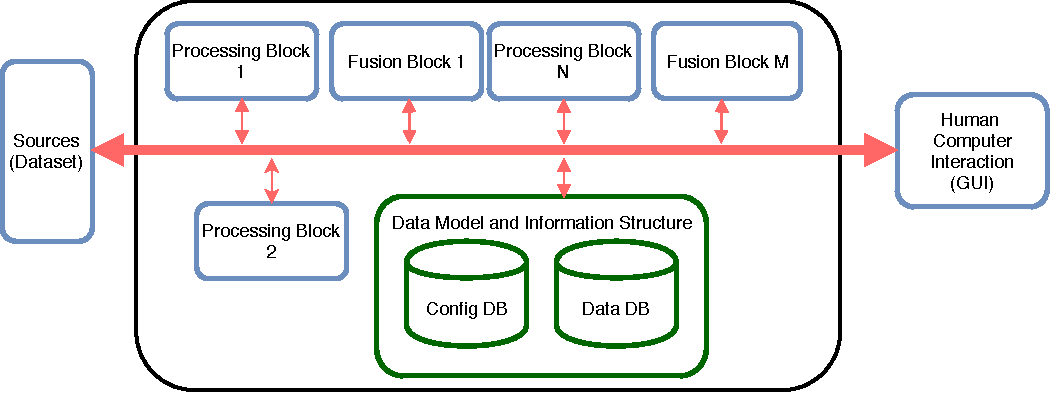
\includegraphics[scale=0.5]{../fig/3/proposal_blocks.pdf}
\caption{General overview of proposed architecture and its components. Red for the communication scheme, green for data model and blue for processing blocks}
\label{proposal_blocks}
\end{figure} 

In order to isolate the processing tasks of the \textit{communication system}, a Publisher-Subscriber approach is selected. The benefits of this option is that data can be shared between diferent blocks without generating a dependency from publishers to subscribers. Another benefit is that exposing a defined mechanism for publishing or subscribing, allows the system to be implementation agnostic.

The \textit{data model} proposed for the system includes the abstraction of the sensing elements and the intersection model. Sensor elements will include the technical parameters and will provide an interface for controlling them and accessing the data generated. The intersection has should be modeled as a unit that includes its geometry properties, traffic direction and the relation with the sensors in it.

The \textit{information structure} will define the way in which configuration and runtime information is stored and exchanged. In order to keep the system language-agnostic and highly integrable, formats like JSON or markup language should be using for static files and established serialisation option are the way to go for data exchanging, because they usually provide APIs for their adoption in different platforms.

Processing blocks in an IMS can be divided into four stages in the processing flow: preprocessing, feature analysis, pattern recognition and situation assessment. To keep the modularity and scalability as principles of the architecture, these block must be isolated processes, exchanging data through the defined communication system and sticking to the data model and the information structure provided. This will also allow that the processes could be sparse across different processing units




\section{Conclusions}

Intersection are complex scenarios that still face efficiency and safety issues, although different approaches have been proposed and implemented. The Internet of things adds a new set of tools for several applications, offering improvements and all the stack of an Intersection Management System application, from the hardware up to the control and user interaction.

Since the establishment of IoT, intersection management system applications have moved from simulated and proposed scenarios to prototype creation and real world deployments, because the creation of sources of data and the implementation of computing systems is not longer expensive as it was 5 or more years ago.

The two main contributions derived from this work is a comprehensive review of intersection management systems and a proposed scalable and modular architecture for traffic monitoring at an intersection enable for its integration with IoT systems.

Oncoming advances in computing capabilities, low-power platforms, and a variety of communication protocols, open a door to newer and optimized solutions. Also, these allow the generation of joint solutions with a wider scope, not just for transportation, but for social or environmental scenarios, having a higher impact on society.


\bibliography{IEEEabrv,../bibliography,iot}



\end{document}
